\documentclass[a4j,dvipdfmx]{jsarticle}
\usepackage{graphicx}
\usepackage{amsmath}
\usepackage{amsfonts}
\usepackage{amssymb}
\usepackage{array}
\usepackage{booktabs}
\usepackage{multirow}
\usepackage{geometry}
\usepackage{listings}
\usepackage{xcolor}
\usepackage{float}
\usepackage{url}
\usepackage{subfigure}

\geometry{a4paper, margin=25mm}

% コードのスタイル設定
\lstset{
    basicstyle=\ttfamily\footnotesize,
    breaklines=true,
    frame=single,
    numbers=left,
    numberstyle=\tiny,
    showstringspaces=false
}

\title{7セグメントディスプレイ論理回路の最適化手法に関する比較研究}
\author{学籍番号: 08D23091 \\ 氏名: 辻 孝弥}
\date{提出日: \today}

\begin{document}

\maketitle

\section{実験背景}

7セグメントディスプレイは、数字やアルファベットを表示するための最も基本的な表示デバイスの一つである。デジタル時計、電卓、各種計測器において広く使用されており、現代のデジタル技術の基礎を成している。

7セグメントディスプレイは、a〜gまでの7つのセグメントから構成され、これらの点灯パターンによって16進数(0〜F)を表現する。各セグメントの制御には論理回路が必要であり、入力となる4ビットの2進数(0000〜1111)に対して、適切な出力パターン(7ビット)を生成する必要がある。

この論理回路の設計において、回路の複雑さとコストを最小化するため、論理式の最簡化が重要な課題となる。論理式の最簡化には複数の手法が存在し、それぞれ異なるアプローチと特徴を持つ。

\section{実験目的}

本実験の目的は以下の通りである:

\begin{enumerate}
\item 16進数表示用7セグメントディスプレイの論理回路を設計し、手動による最簡化を行う
\item 異なる最適化手法(手動カルノー図法、CPLEX線形計画法、クワイン・マクラスキー法)による結果を比較分析する
\item 各手法の特徴と差異が生じる理由を理論的に考察する
\item クワイン・マクラスキー法の計算複雑性を実証し、入力ビット数増加による指数関数的増大を確認する
\end{enumerate}

\section{実験の理論}

\subsection{7セグメントディスプレイの原理}

7セグメントディスプレイは7つのセグメント(a, b, c, d, e, f, g)から構成される。4ビット入力($X_1, X_2, X_3, X_4$)に対して、各セグメントの点灯状態を決定する論理関数を求める必要がある。

\subsection{論理最簡化手法}

\subsubsection{カルノー図法}
カルノー図法は、真理値表を2次元のマップ上に配置し、隣接する1のグループを視覚的に識別することで最簡主加法標準形を求める手法である。4変数の場合、$4 \times 4$のマップを使用し、以下の手順で最簡化を行う:

\begin{enumerate}
\item 真理値表から出力が1となる最小項をカルノー図上にマッピング
\item 隣接する1のセルをグループ化(1個、2個、4個、8個の2の累乗単位)
\item 各グループから論理項を導出
\item 全ての最小項をカバーする最小の論理項集合を選択
\end{enumerate}

\subsubsection{線形計画法(CPLEX)}
CPLEXを用いた最適化では、論理式の最簡化を整数線形計画問題として定式化する。目的関数を使用する論理項の数の最小化とし、制約条件として全ての最小項をカバーすることを設定する。

\subsubsection{クワイン・マクラスキー法}
クワイン・マクラスキー法は以下の2段階から構成される:
\begin{enumerate}
\item \textbf{素項の生成}:最小項を1の数によってグループ化し、隣接グループの項を結合して素項を生成
\item \textbf{Petrick's Method}:素項の中から最小カバーを選択
\end{enumerate}

\section{実験結果}

\subsection{課題1:真理値表の完成と論理回路設計}

\subsubsection{真理値表(表2.1)}

表\ref{tab:truth_table}に16進数表示用7セグメントディスプレイの完全な真理値表を示す。

\begin{table}[H]
\centering
\caption{7セグメントディスプレイの真理値表(表2.1)}
\label{tab:truth_table}
\begin{tabular}{|c|c|c|}
\hline
入力 (4bit) & 表示 & 出力 (abcdefg) \\
\hline
0000 & 0 & 1111110 \\
0001 & 1 & 0110000 \\
0010 & 2 & 1101101 \\
0011 & 3 & 1111001 \\
0100 & 4 & 0110011 \\
0101 & 5 & 1011011 \\
0110 & 6 & 1011111 \\
0111 & 7 & 1110000 \\
1000 & 8 & 1111111 \\
1001 & 9 & 1111011 \\
1010 & A & 1110111 \\
1011 & b & 0011111 \\
1100 & C & 1001110 \\
1101 & d & 0111101 \\
1110 & E & 1001111 \\
1111 & F & 1000111 \\
\hline
\end{tabular}
\end{table}

\subsubsection{カルノー図による導出過程}

各セグメントについて、カルノー図を用いた詳細な導出過程を示す。

\textbf{セグメントaの導出例:}

セグメントaが点灯する入力は:0, 2, 3, 5, 6, 7, 8, 9, A, C, E, F(12個の最小項)

4変数カルノー図において、変数配置を以下のように設定:
\begin{itemize}
\item 横軸:$X_3X_4$(00, 01, 11, 10の順)
\item 縦軸:$X_1X_2$(00, 01, 11, 10の順)
\end{itemize}

カルノー図上で1となるセルをマッピングし、隣接する1のグループを特定:

\begin{enumerate}
\item グループ1:$(X_1X_2X_3X_4) = 00\_0, 01\_0, 10\_0$ → $\overline{X_2} \cdot \overline{X_4}$
\item グループ2:$(X_1X_2X_3X_4) = 0\_1\_$ → $\overline{X_1} \cdot X_3$
\item グループ3:$(X_1X_2X_3X_4) = \_11\_$ → $X_2 \cdot X_3$
\item グループ4:$(X_1X_2X_3X_4) = 0101$ → $\overline{X_1} \cdot X_2 \cdot X_4$
\item グループ5:$(X_1X_2X_3X_4) = 1\_\_0$ → $X_1 \cdot \overline{X_4}$
\item グループ6:$(X_1X_2X_3X_4) = 1000$ → $X_1 \cdot \overline{X_2} \cdot \overline{X_3}$
\end{enumerate}

したがって、セグメントaの最簡論理式は:
$$a = \overline{X_2} \cdot \overline{X_4} + \overline{X_1} \cdot X_3 + X_2 \cdot X_3 + \overline{X_1} \cdot X_2 \cdot X_4 + X_1 \cdot \overline{X_4} + X_1 \cdot \overline{X_2} \cdot \overline{X_3}$$

\subsubsection{カルノー図による導出}

図\ref{fig:karnaugh_maps_abc}〜\ref{fig:karnaugh_maps_g}に各セグメント(a〜g)のカルノー図を示す。これらの図は、上記の論理式導出過程における最小項のグループ化を視覚的に表現したものである。

\begin{figure}[H]
\centering
\subfigure[セグメントa]{
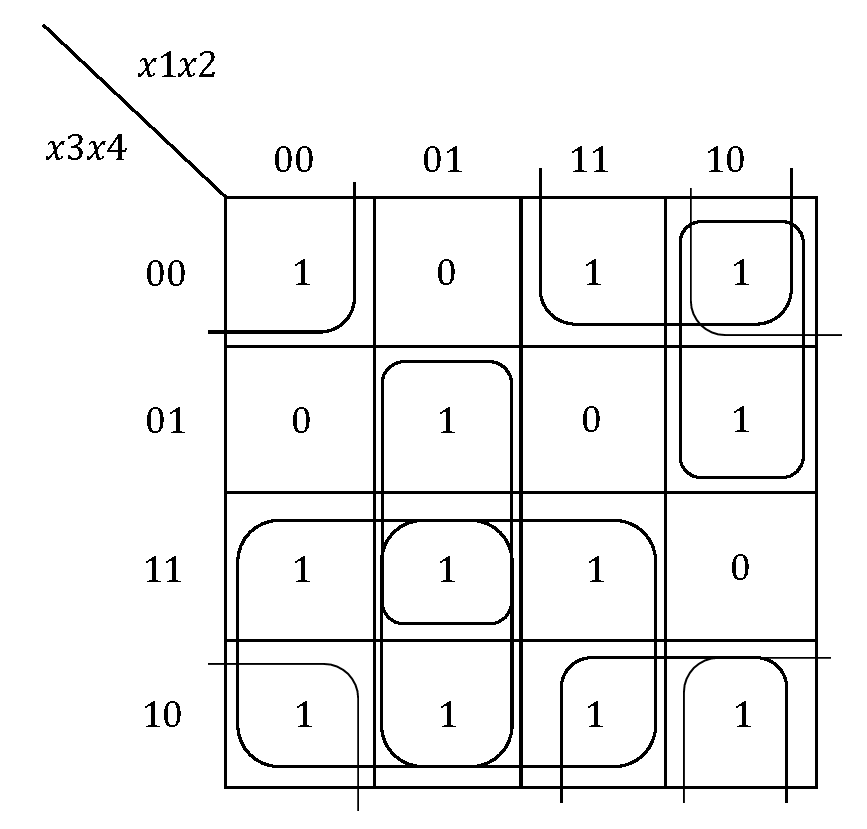
\includegraphics[width=0.31\textwidth]{resources/karnaugh/a.pdf}
}
\subfigure[セグメントb]{
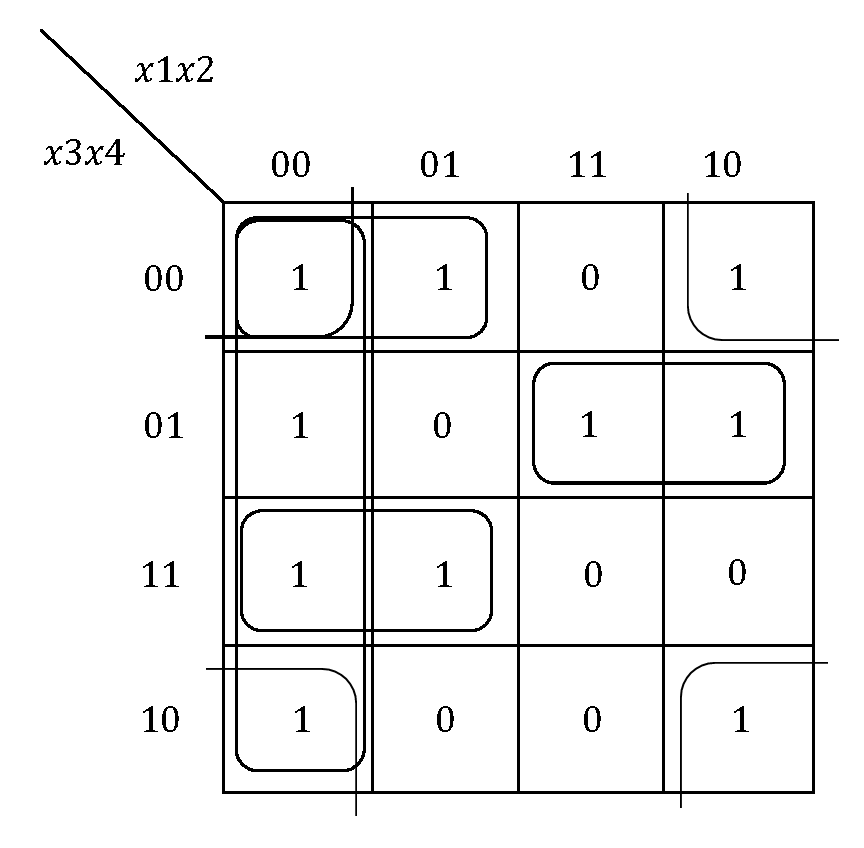
\includegraphics[width=0.31\textwidth]{resources/karnaugh/b.pdf}
}
\subfigure[セグメントc]{
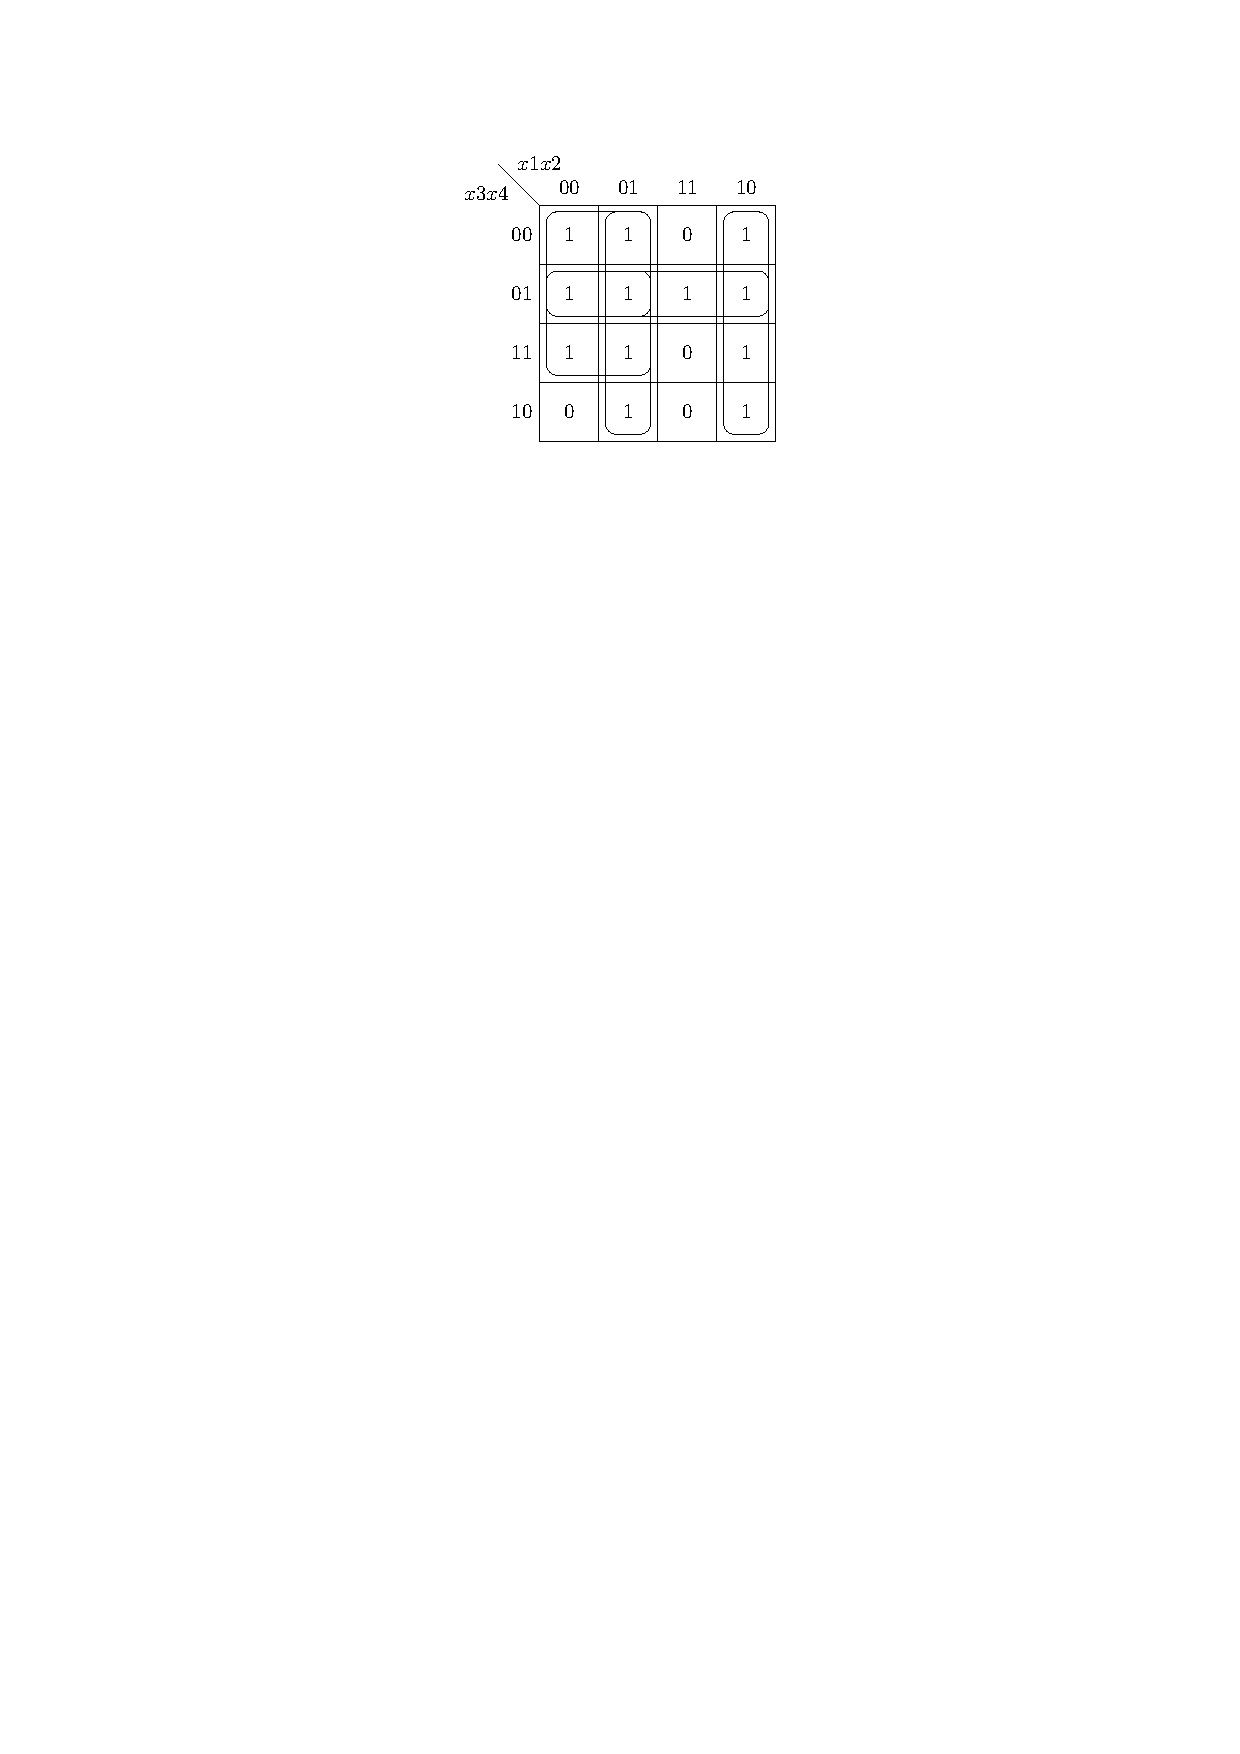
\includegraphics[width=0.31\textwidth]{resources/karnaugh/c.pdf}
}
\caption{カルノー図(a, b, c)}
\label{fig:karnaugh_maps_abc}
\end{figure}

\begin{figure}[H]
\centering
\subfigure[セグメントd]{
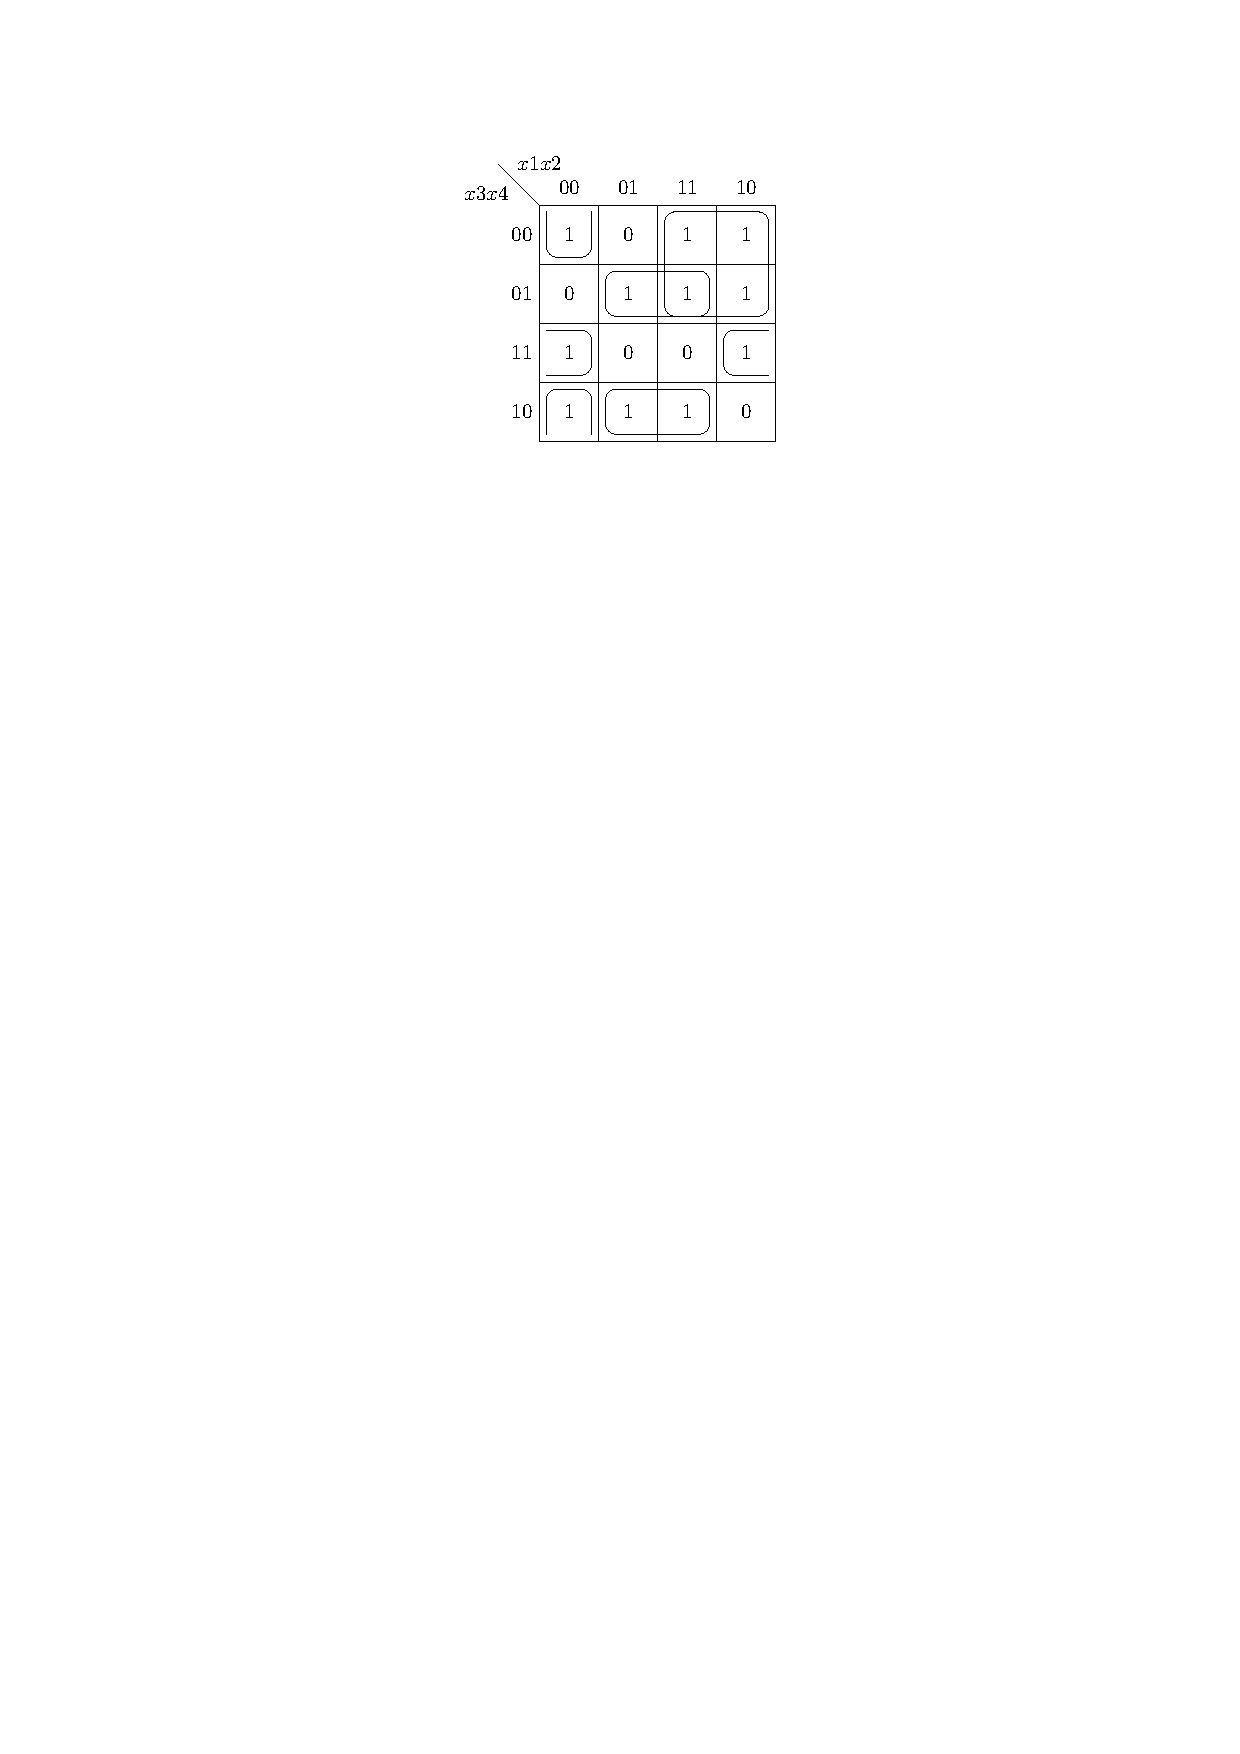
\includegraphics[width=0.31\textwidth]{resources/karnaugh/d.pdf}
}
\subfigure[セグメントe]{
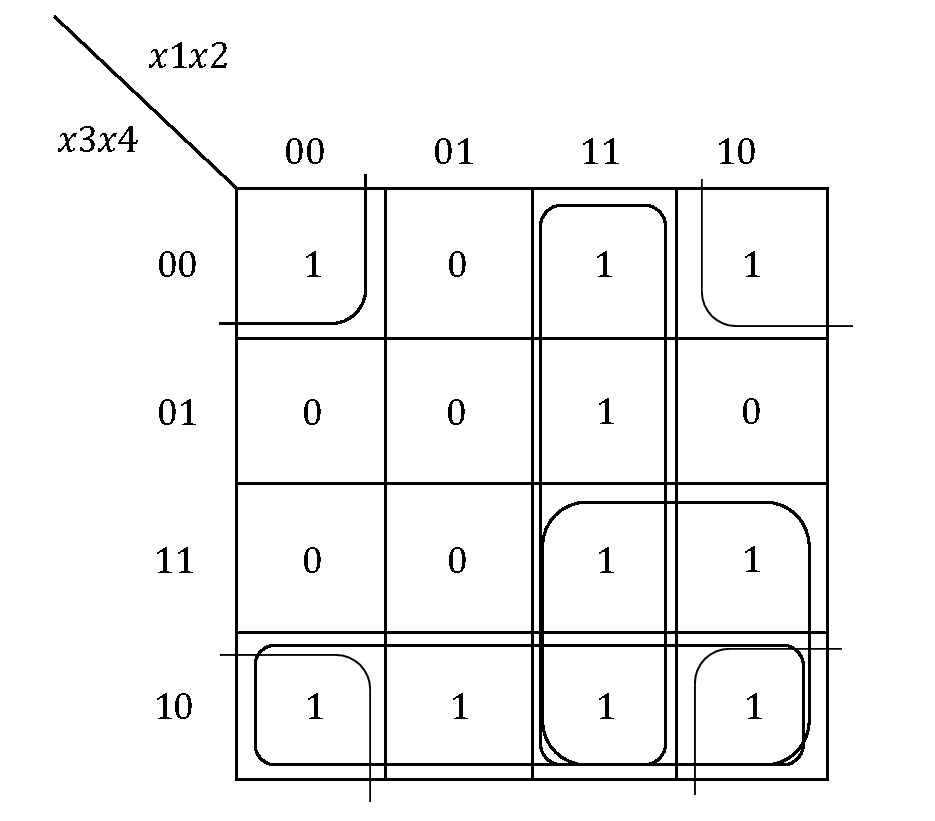
\includegraphics[width=0.31\textwidth]{resources/karnaugh/e.pdf}
}
\subfigure[セグメントf]{
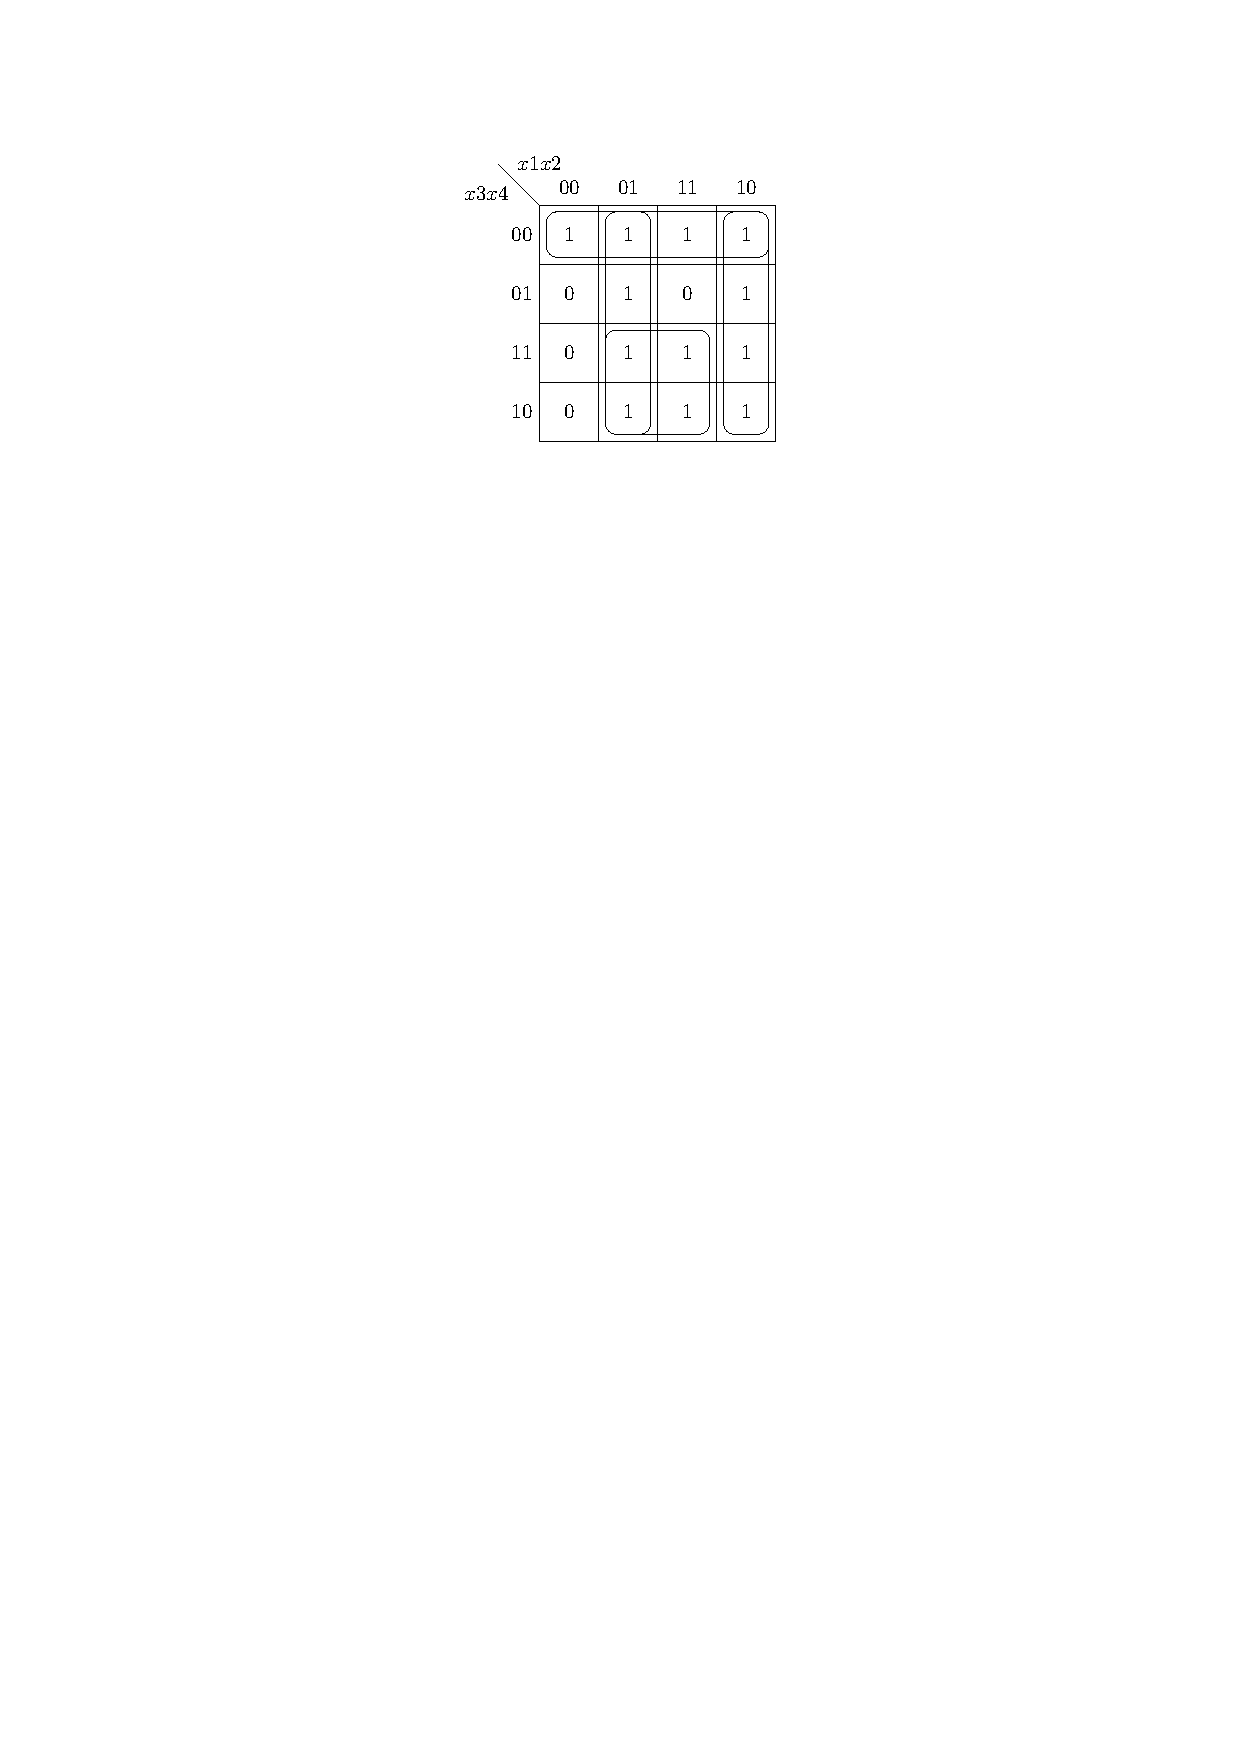
\includegraphics[width=0.31\textwidth]{resources/karnaugh/f.pdf}
}
\caption{カルノー図(d, e, f)}
\label{fig:karnaugh_maps_def}
\end{figure}

\begin{figure}[H]
\centering
\subfigure[セグメントg]{
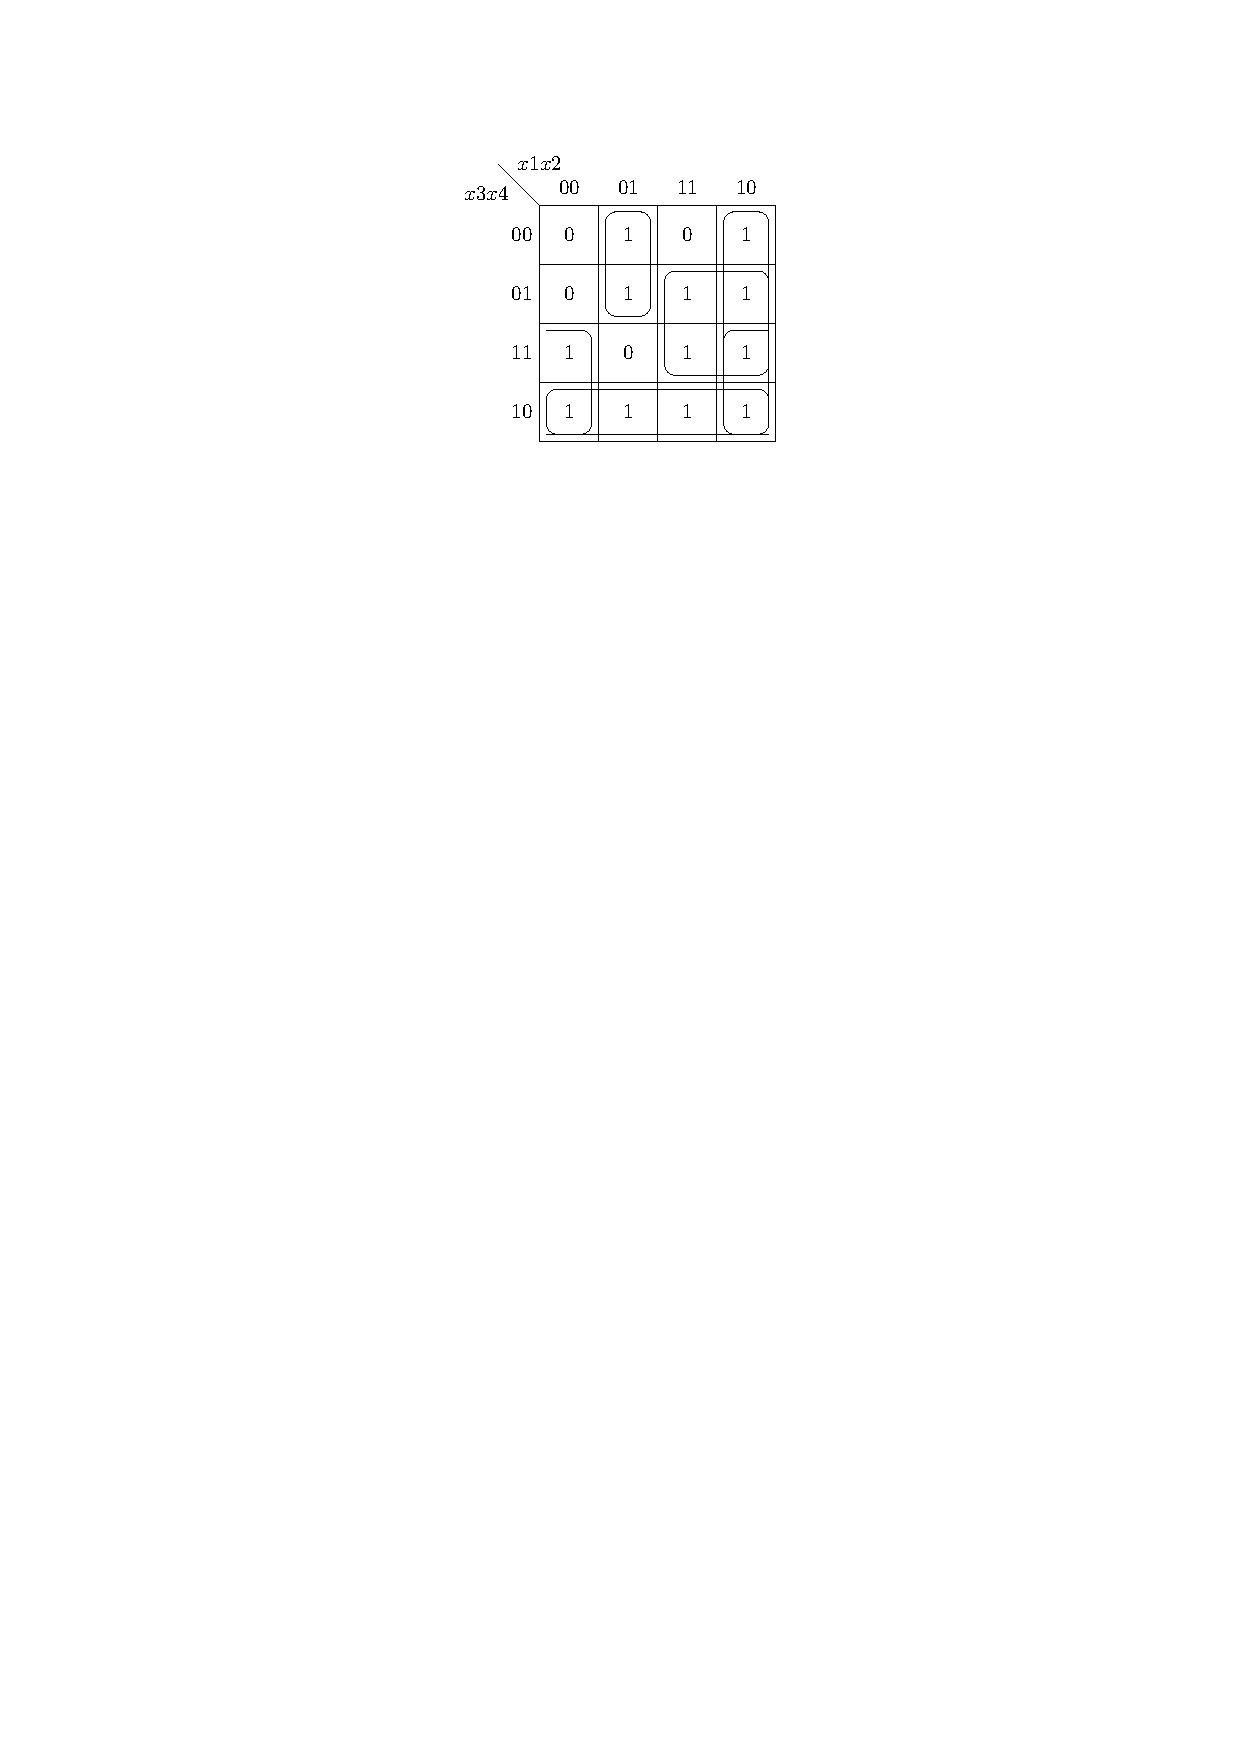
\includegraphics[width=0.45\textwidth]{resources/karnaugh/g.pdf}
}
\caption{カルノー図(g)}
\label{fig:karnaugh_maps_g}
\end{figure}

同様の手順により、全セグメントの論理式を導出した:

\begin{align}
a &= \overline{X_2} \cdot \overline{X_4} + \overline{X_1} \cdot X_3 + X_2 \cdot X_3 + \overline{X_1} \cdot X_2 \cdot X_4 + X_1 \cdot \overline{X_4} + X_1 \cdot \overline{X_2} \cdot \overline{X_3} \\
b &= \overline{X_2} \cdot \overline{X_4} + \overline{X_1} \cdot \overline{X_2} + \overline{X_1} \cdot \overline{X_3} \cdot \overline{X_4} + X_1 \cdot \overline{X_3} \cdot X_4 + \overline{X_1} \cdot X_3 \cdot X_4 \\
c &= \overline{X_1} \cdot \overline{X_3} + \overline{X_1} \cdot X_4 + \overline{X_3} \cdot X_4 + \overline{X_1} \cdot X_2 + X_1 \cdot \overline{X_2} \\
d &= \overline{X_1} \cdot \overline{X_2} \cdot \overline{X_4} + X_1 \cdot \overline{X_3} + X_2 \cdot \overline{X_3} \cdot X_4 + \overline{X_2} \cdot X_3 \cdot X_4 + X_2 \cdot X_3 \cdot \overline{X_4} \\
e &= \overline{X_2} \cdot \overline{X_4} + X_1 \cdot X_2 + X_1 \cdot X_3 + X_3 \cdot \overline{X_4} \\
f &= \overline{X_3} \cdot \overline{X_4} + \overline{X_1} \cdot X_2 + X_1 \cdot \overline{X_2} + X_2 \cdot X_3 \\
g &= \overline{X_1} \cdot X_2 \cdot \overline{X_3} + X_1 \cdot \overline{X_2} + X_1 \cdot X_4 + \overline{X_2} \cdot X_3 + X_3 \cdot \overline{X_4}
\end{align}

\newpage

\subsubsection{論理回路図}

上記の論理式に基づき、AND、OR、NOTゲートのみを用いた論理回路を設計した。図\ref{fig:segment_circuits_abc}〜\ref{fig:segment_circuits_g}に各セグメントの個別回路を、図\ref{fig:complete_circuit}に全体回路を示す。


\begin{figure}[H]
\centering
\subfigure[セグメントa回路]{
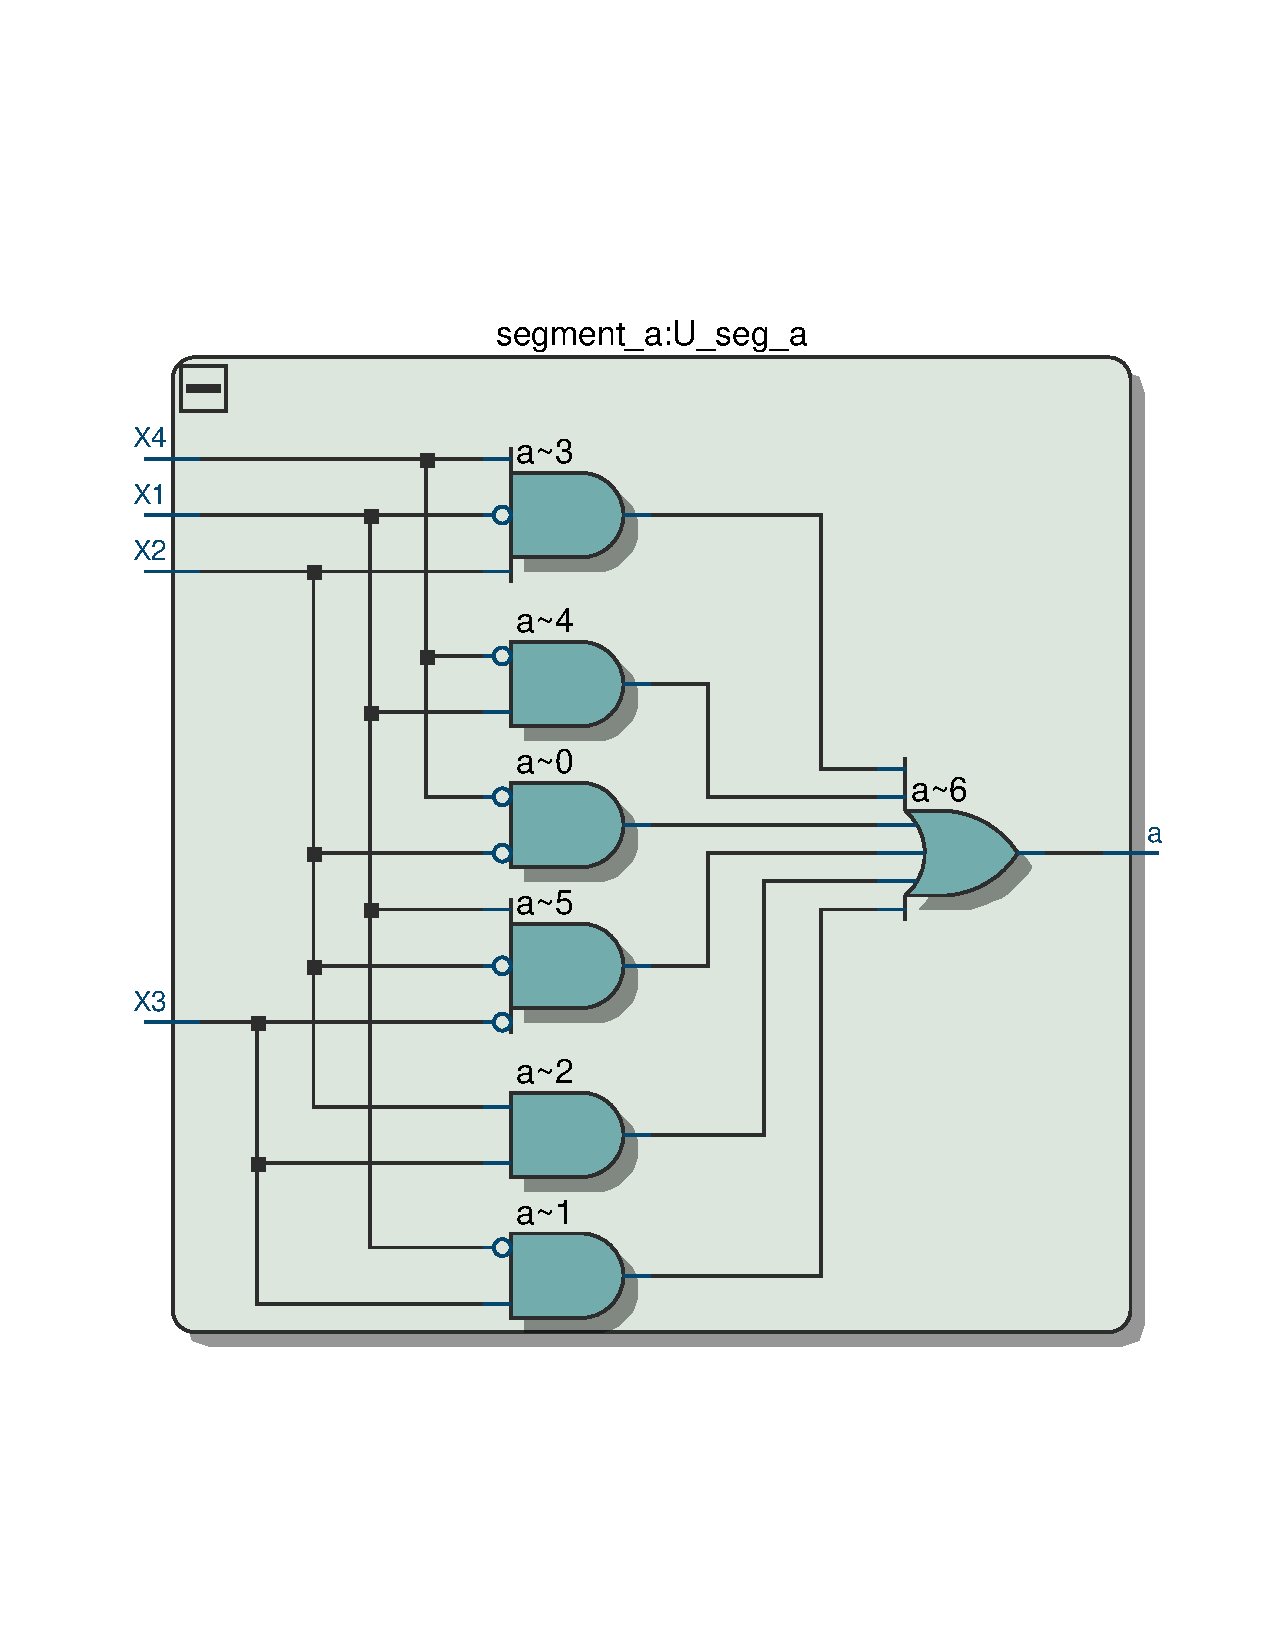
\includegraphics[width=0.31\textwidth]{resources/circuit/segment_a_circuit.pdf}
}
\subfigure[セグメントb回路]{
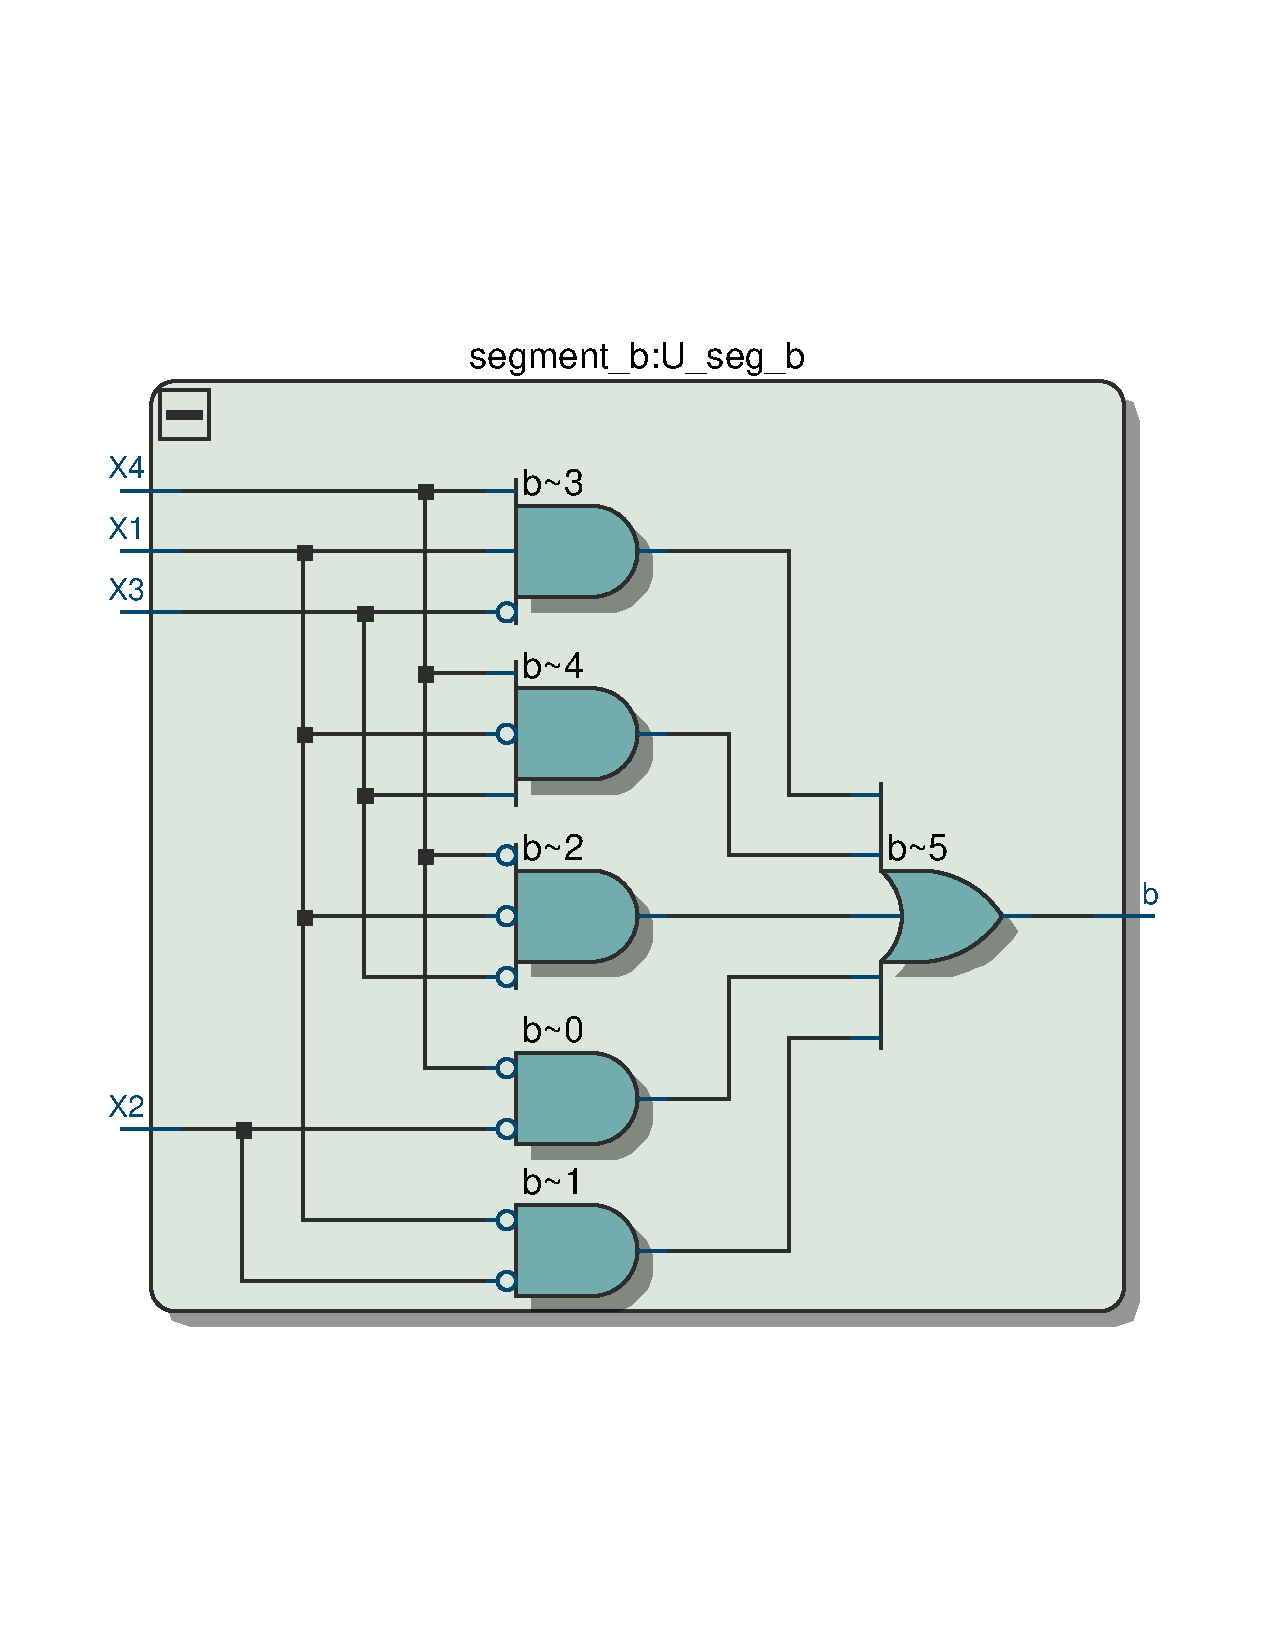
\includegraphics[width=0.31\textwidth]{resources/circuit/segment_b_circuit.pdf}
}
\subfigure[セグメントc回路]{
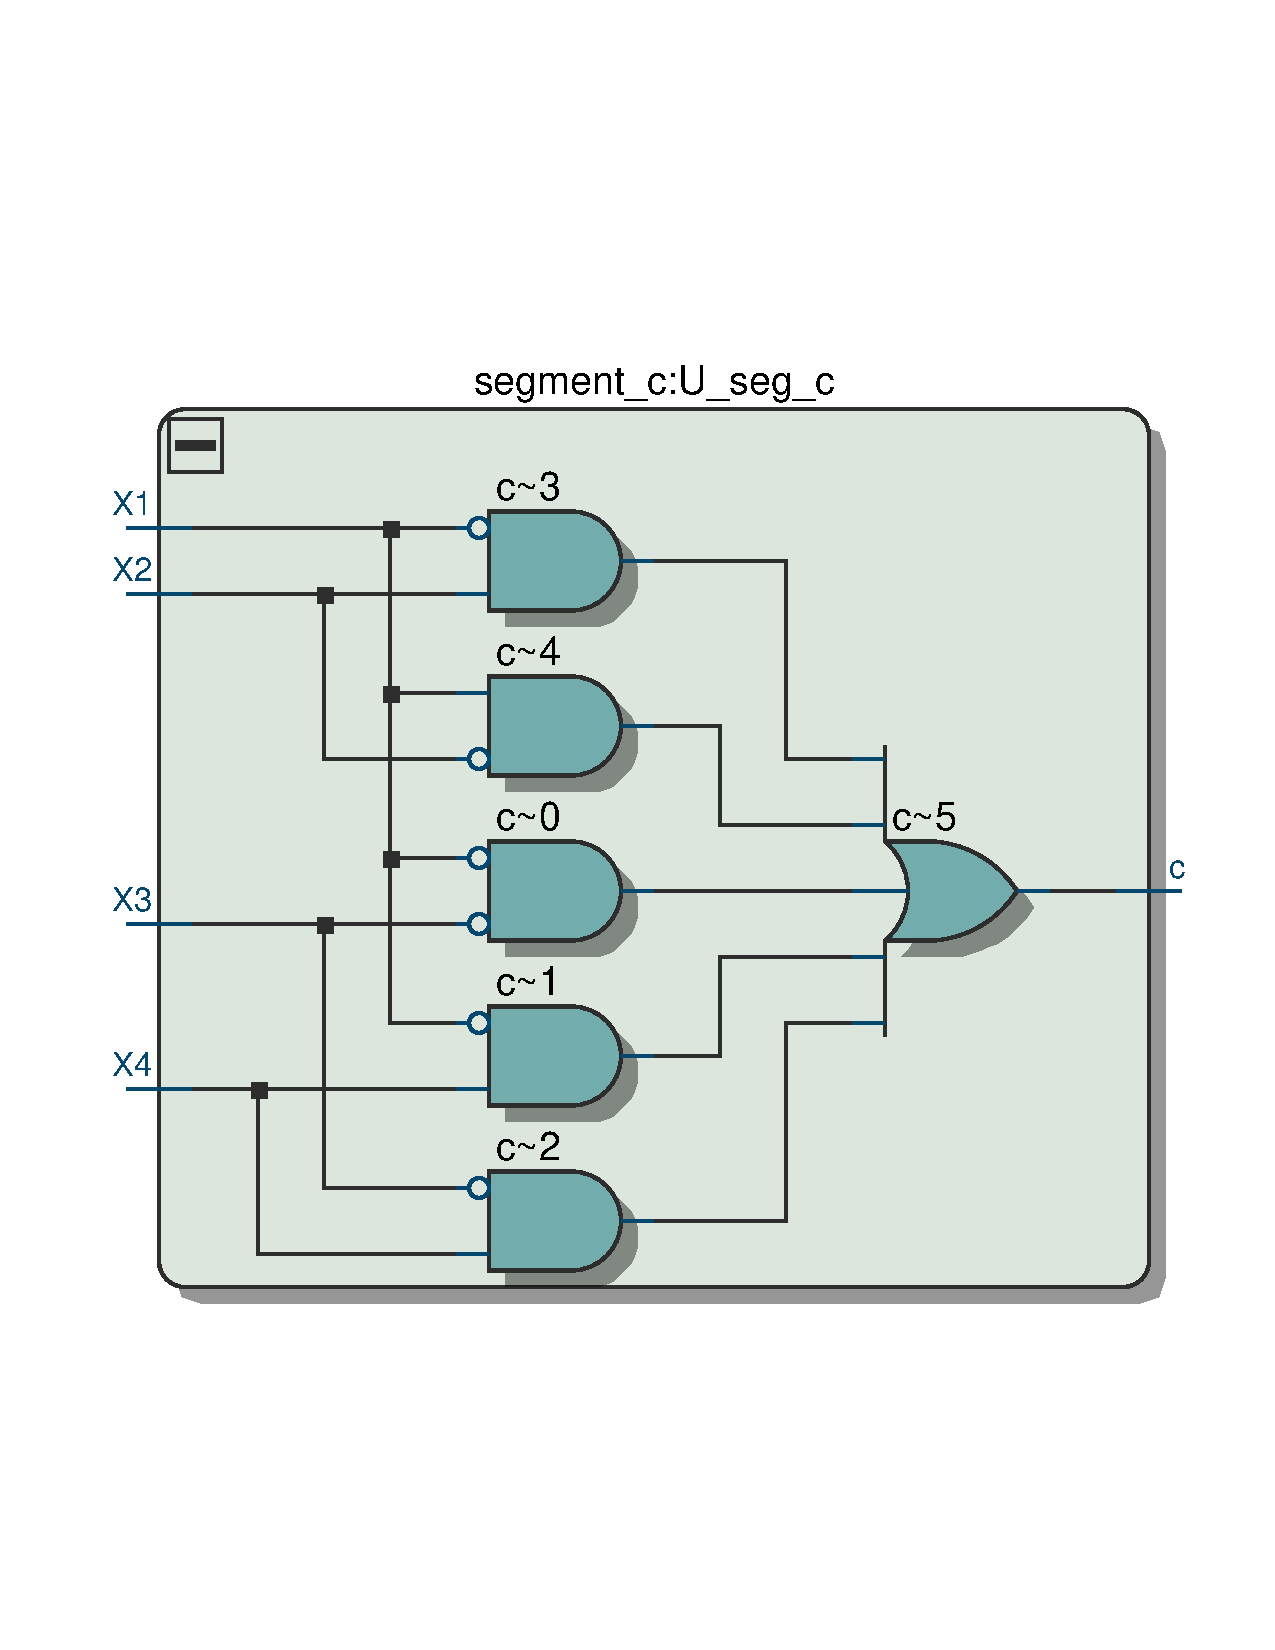
\includegraphics[width=0.31\textwidth]{resources/circuit/segment_c_circuit.pdf}
}
\caption{セグメント個別回路(a, b, c)}
\label{fig:segment_circuits_abc}
\end{figure}

\begin{figure}[H]
\centering
\subfigure[セグメントd回路]{
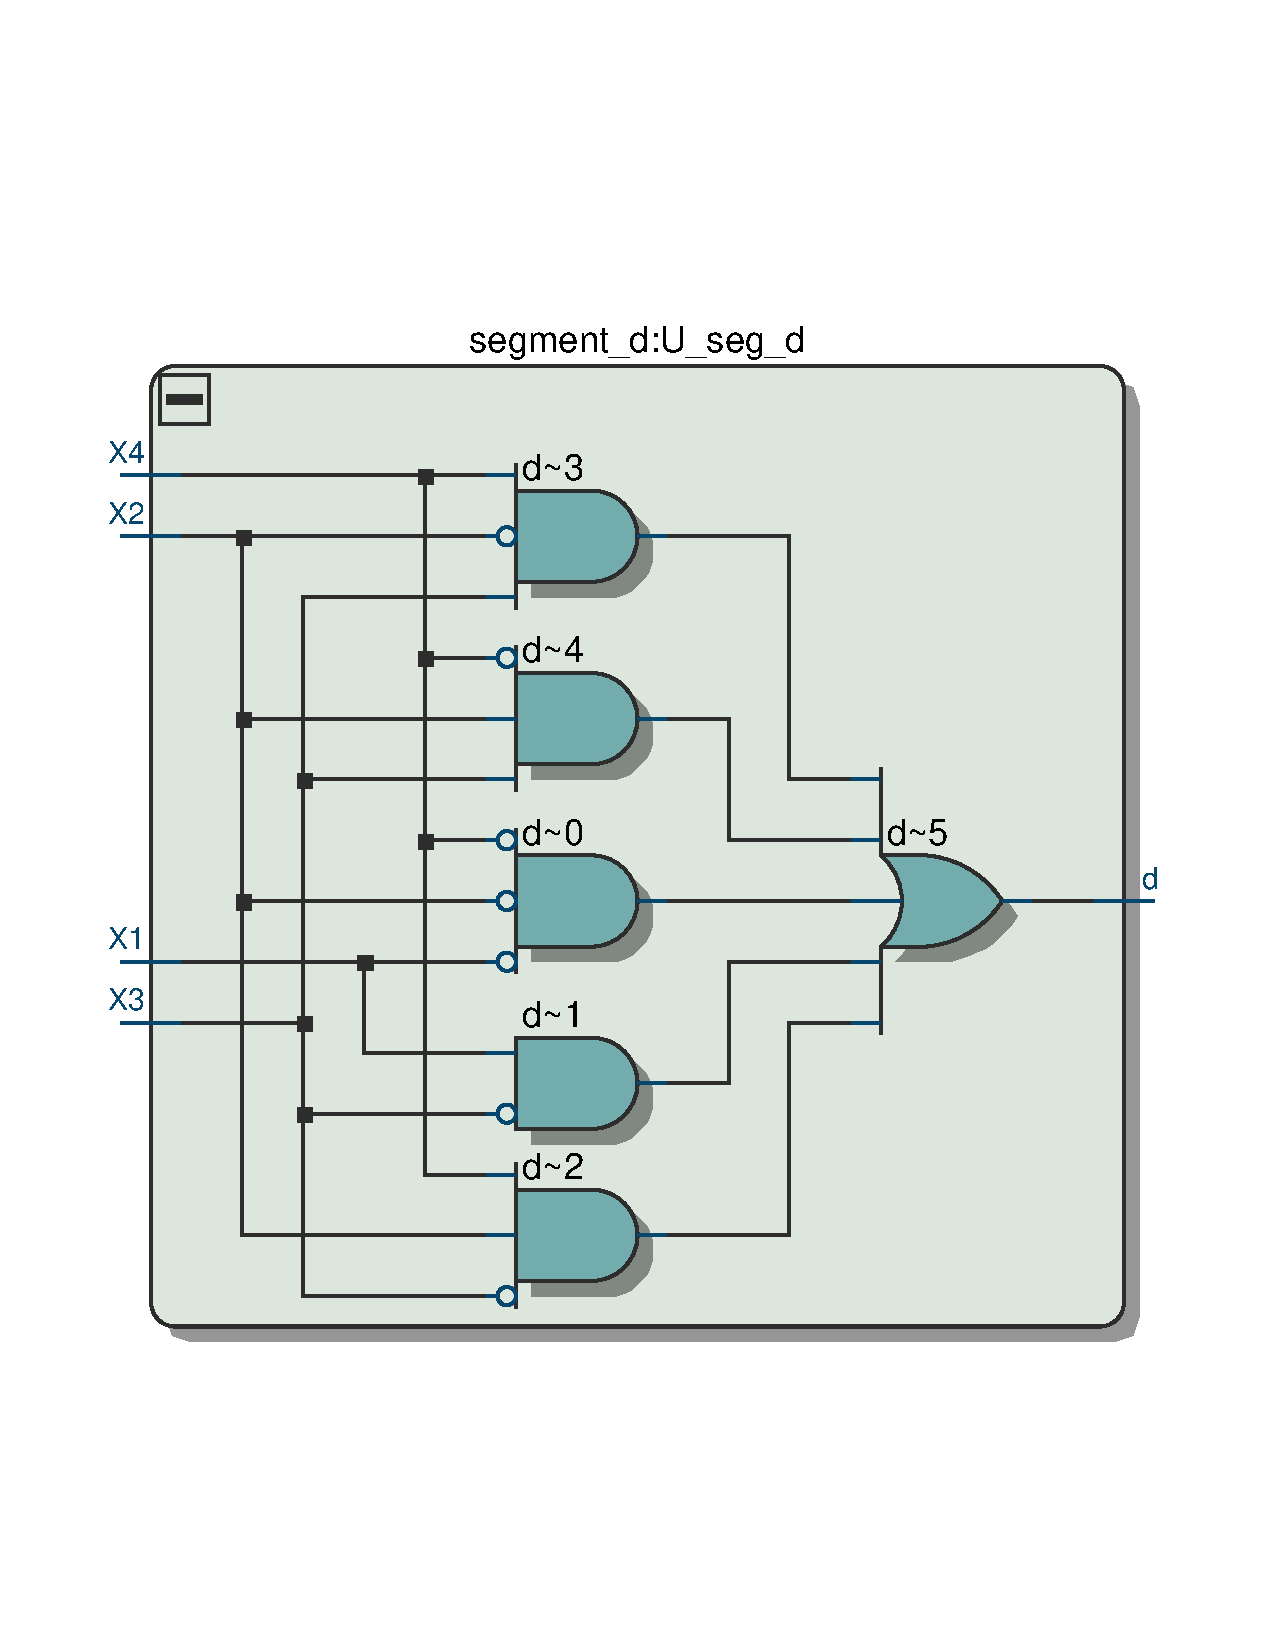
\includegraphics[width=0.31\textwidth]{resources/circuit/segment_d_circuit.pdf}
}
\subfigure[セグメントe回路]{
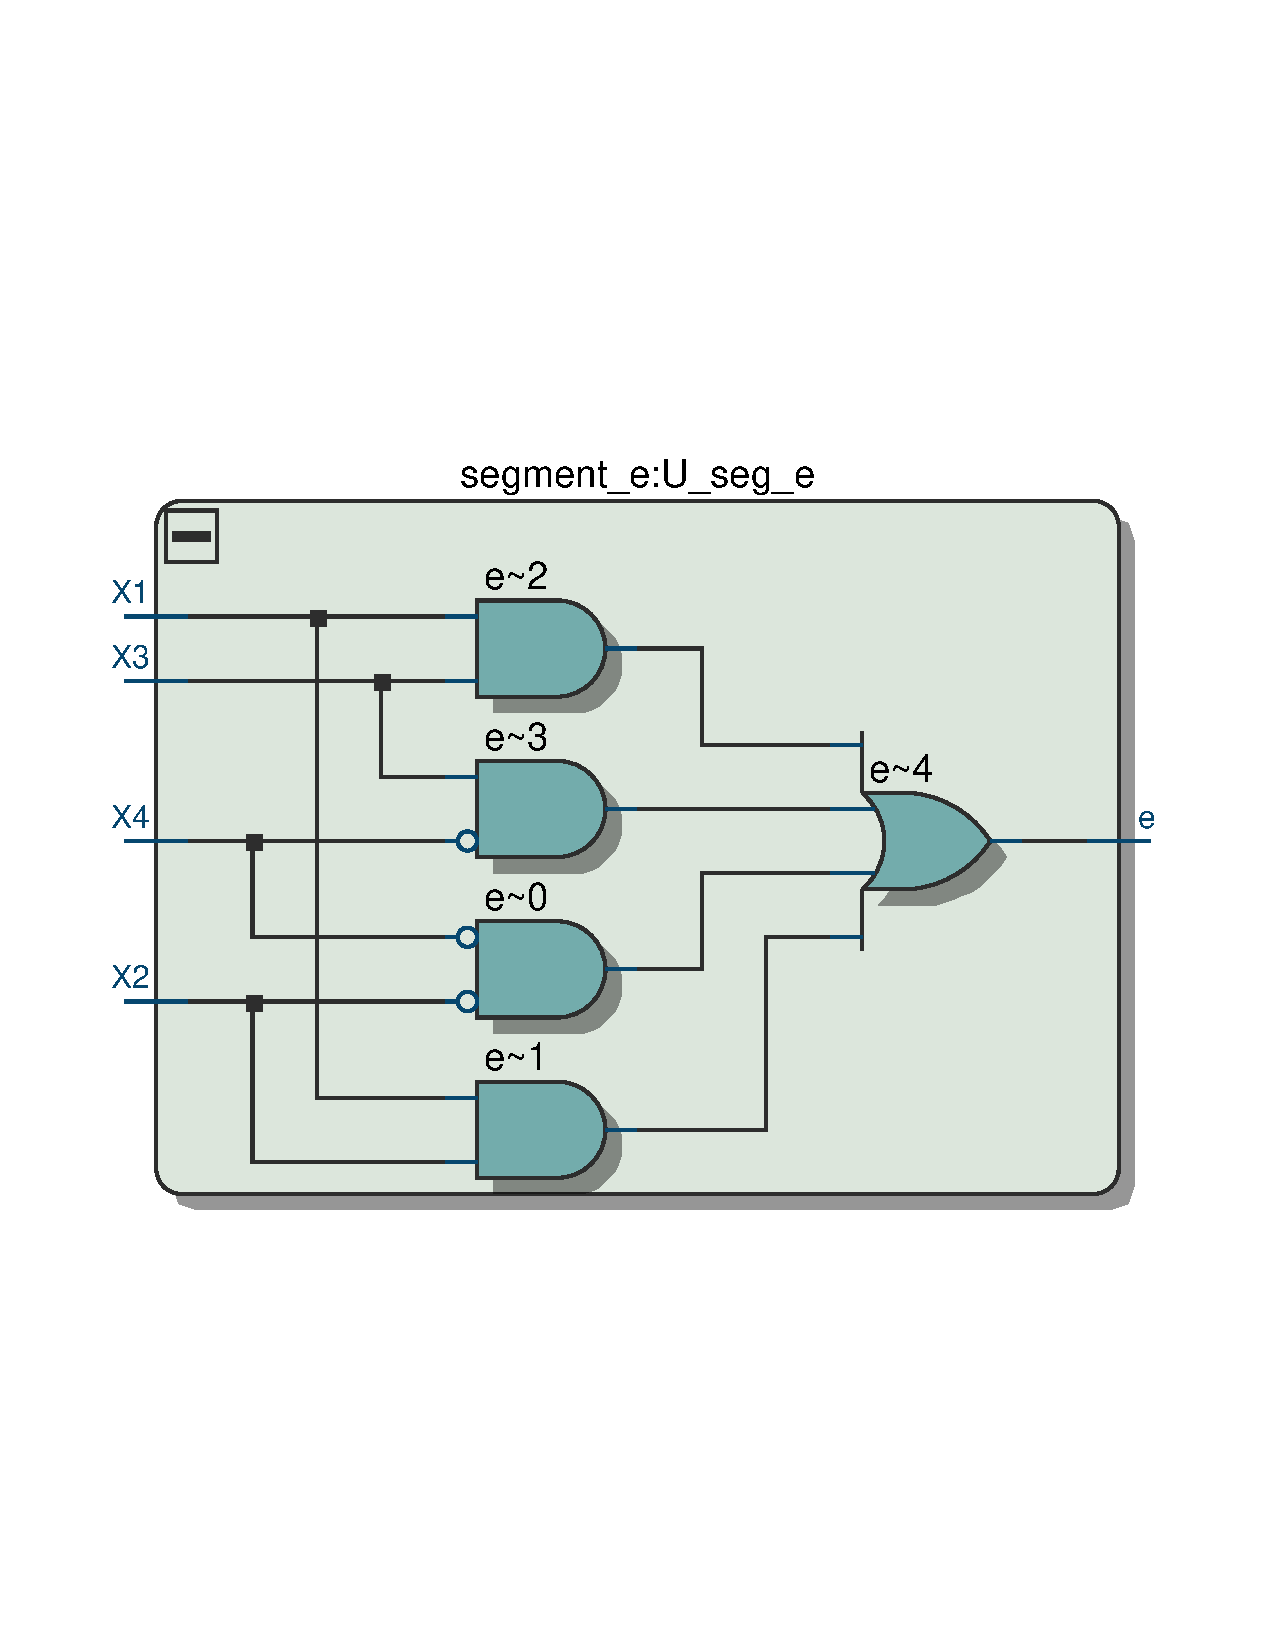
\includegraphics[width=0.31\textwidth]{resources/circuit/segment_e_circuit.pdf}
}
\subfigure[セグメントf回路]{
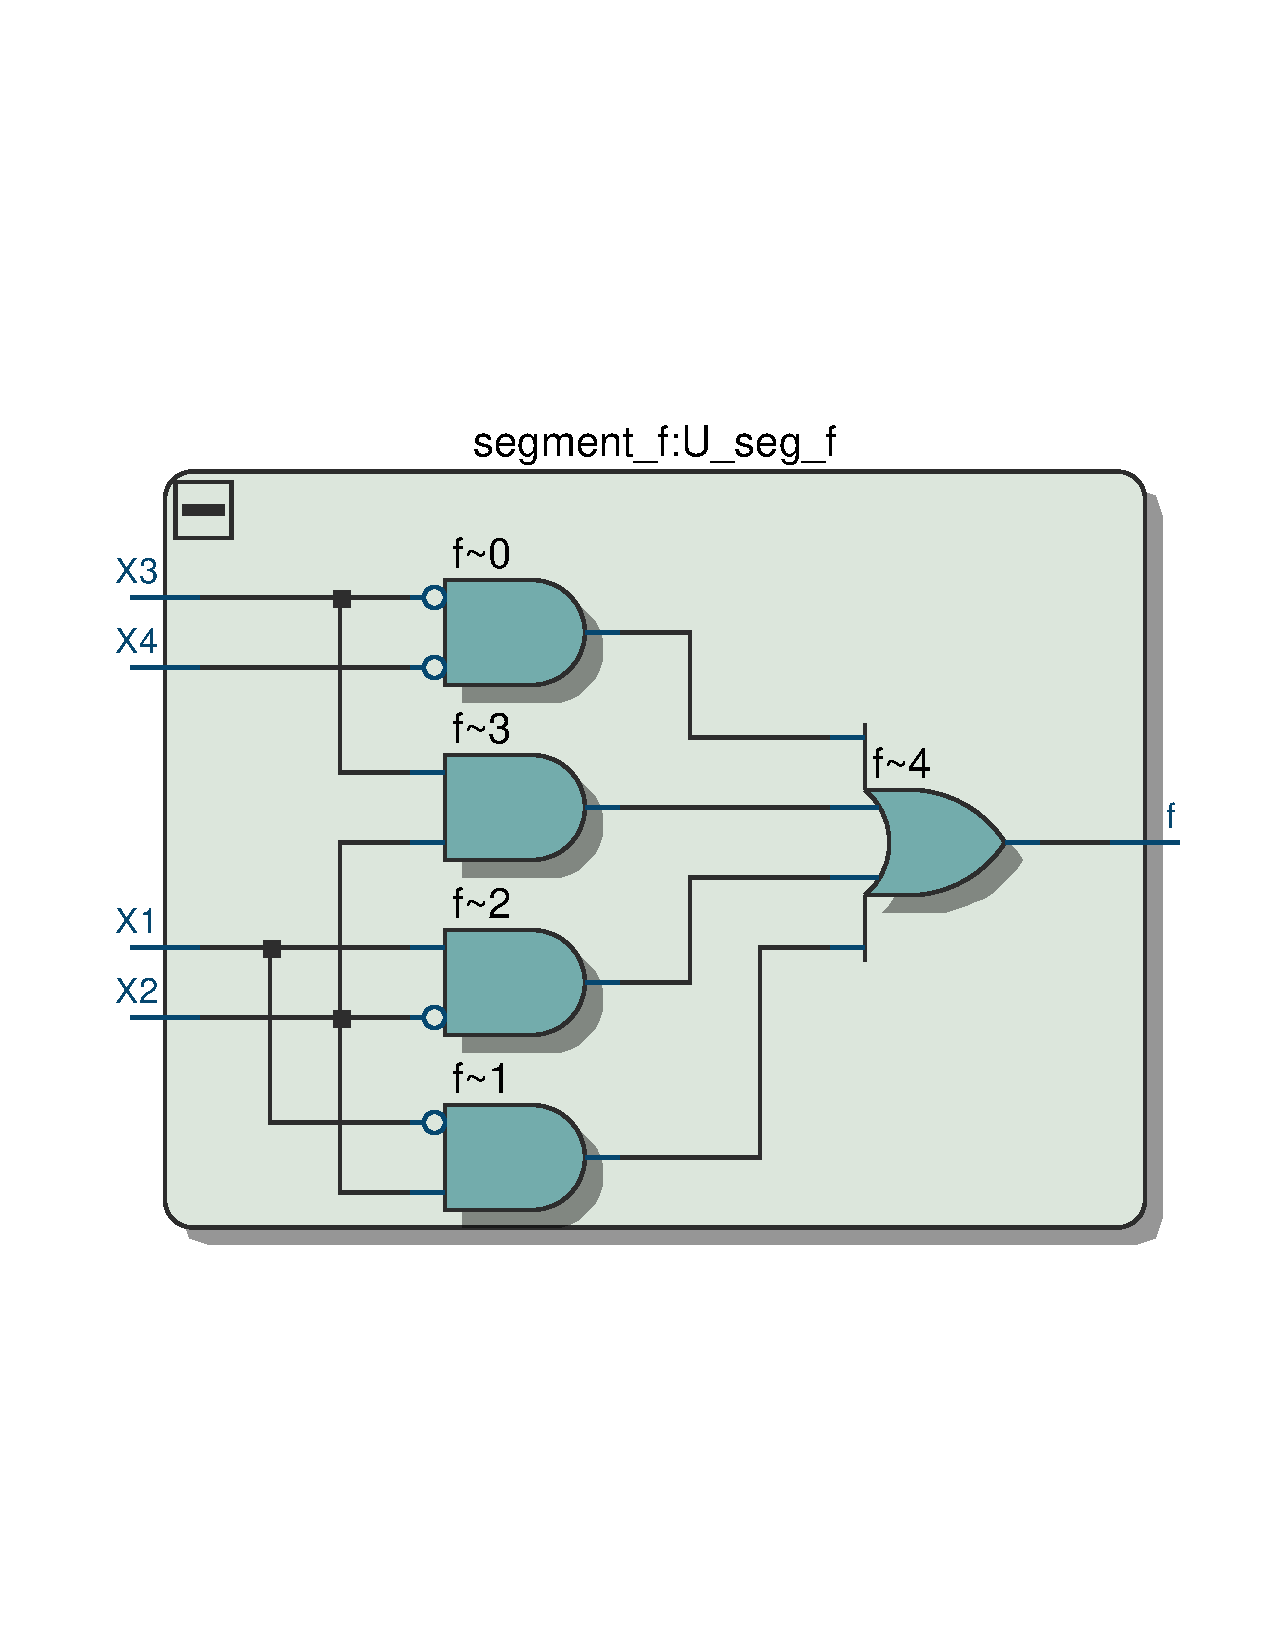
\includegraphics[width=0.31\textwidth]{resources/circuit/segment_f_circuit.pdf}
}
\caption{セグメント個別回路(d, e, f)}
\label{fig:segment_circuits_def}
\end{figure}

\begin{figure}[H]
\centering
\subfigure[セグメントg回路]{
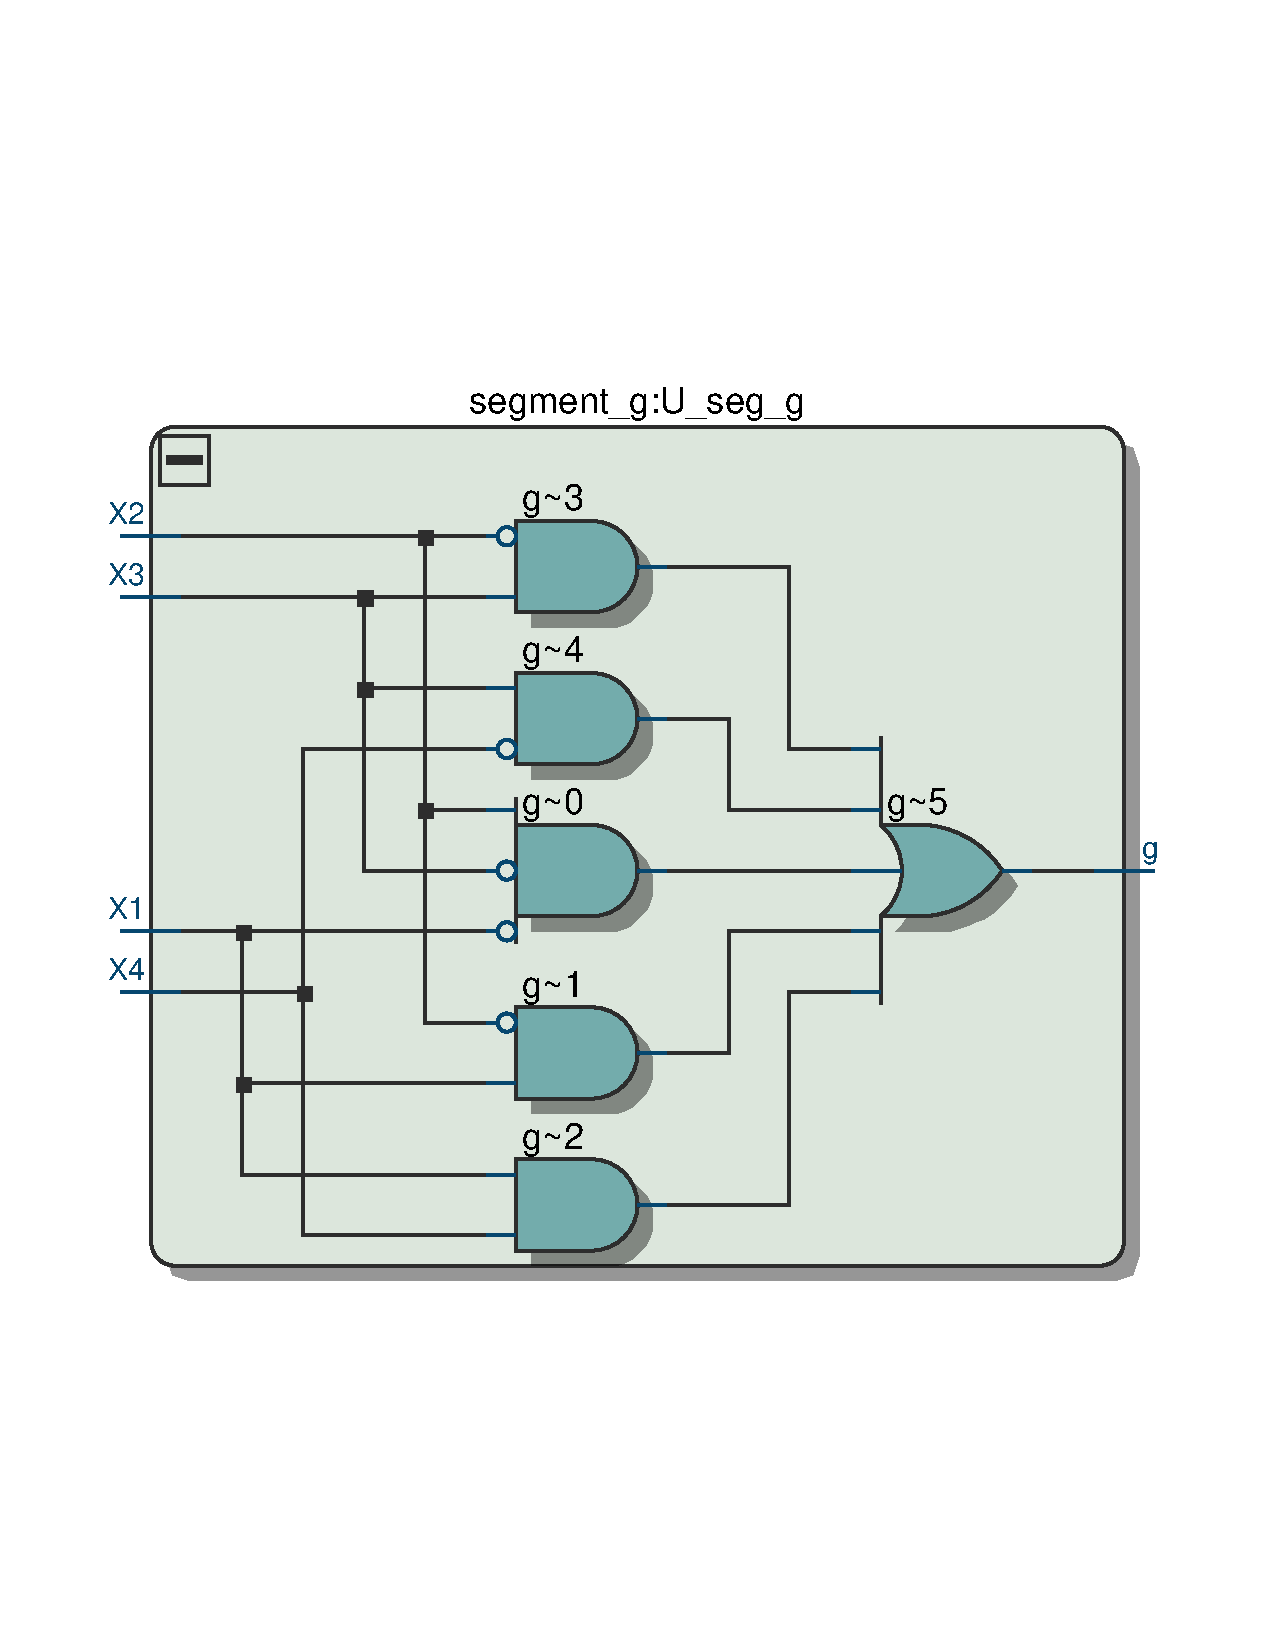
\includegraphics[width=0.45\textwidth]{resources/circuit/segment_g_circuit.pdf}
}
\caption{セグメント個別回路(g)}
\label{fig:segment_circuits_g}
\end{figure}

\begin{figure}[H]
\centering
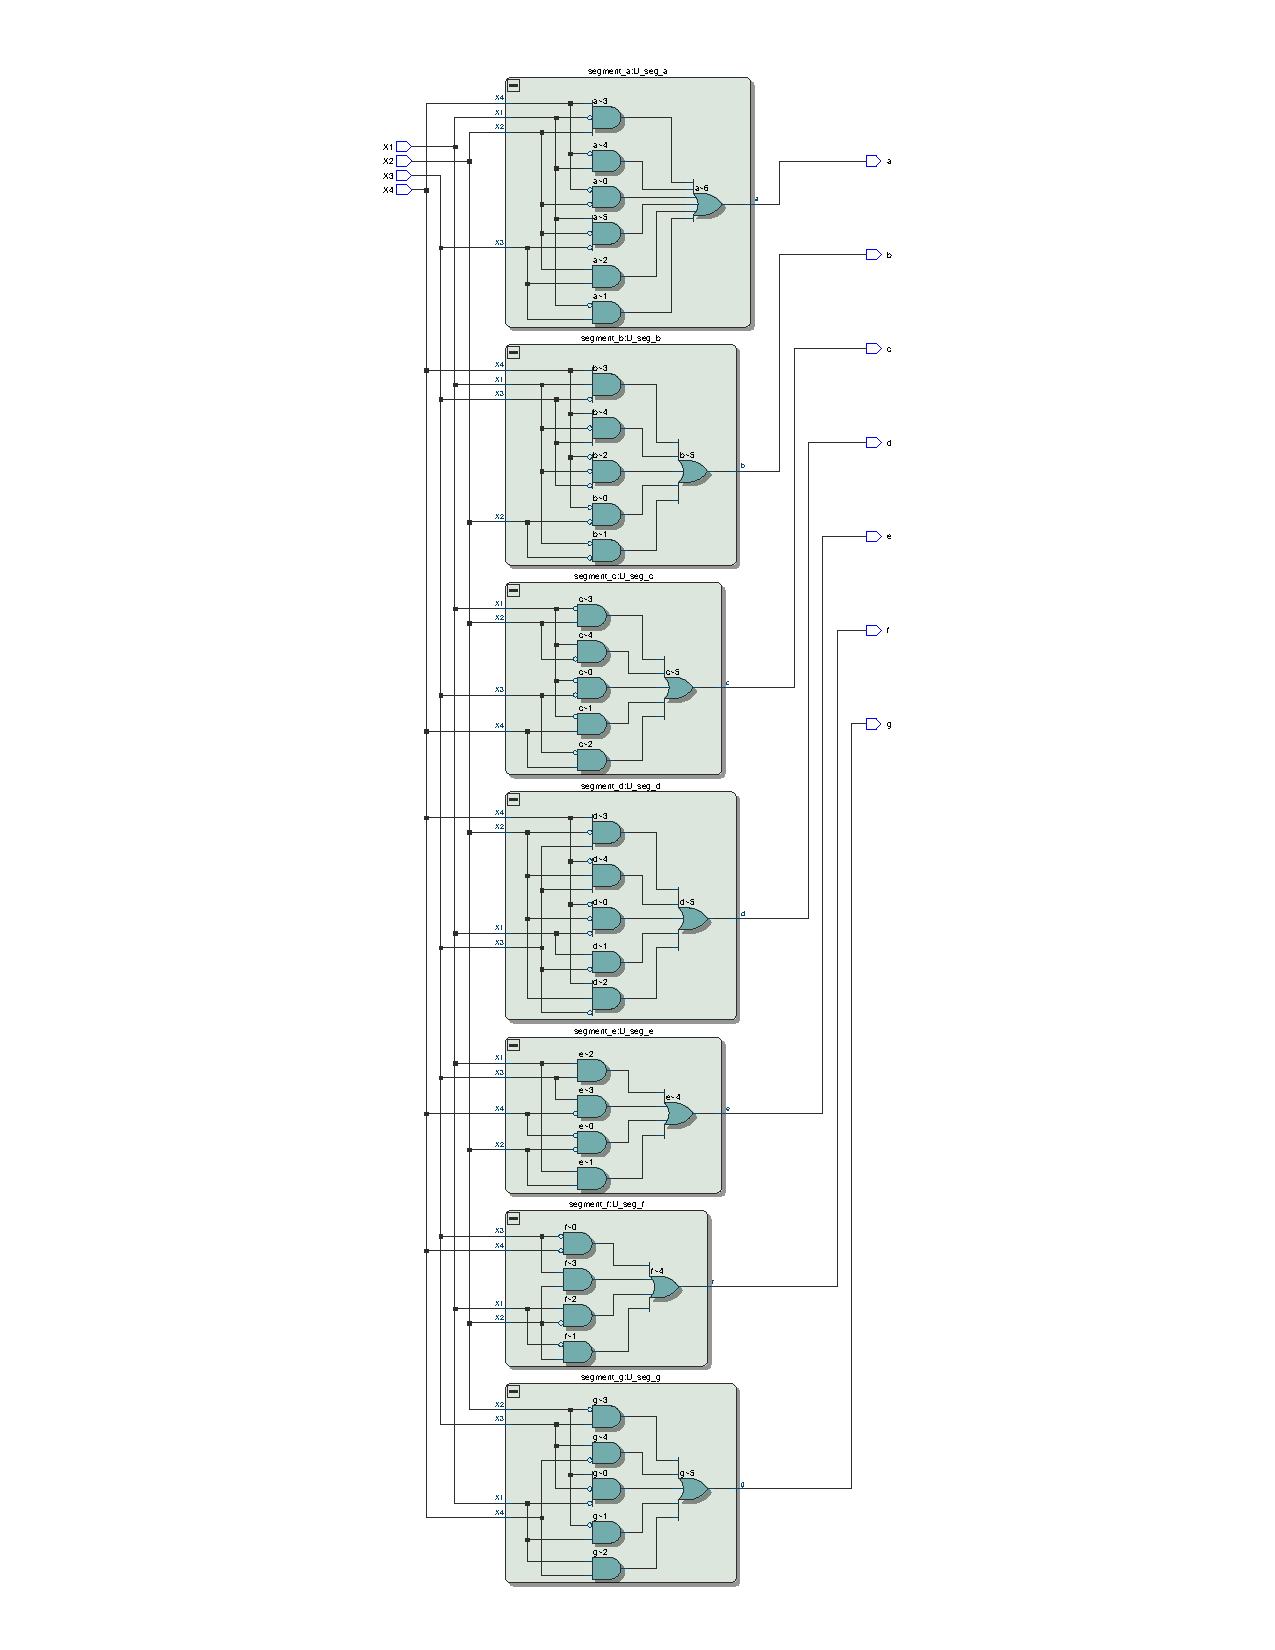
\includegraphics[width=1.1\textwidth]{resources/circuit/seven_segment_circuit_open.pdf}
\caption{7セグメントディスプレイ完全回路図}
\label{fig:complete_circuit}
\end{figure}

\subsection{課題2:最適化手法の比較}

\subsubsection{CPLEX最適化との比較}

表\ref{tab:comparison}に手動導出とCPLEX最適化、クワイン・マクラスキー法による結果の比較を示す。

\begin{table}[H]
\centering
\caption{最適化手法の比較結果}
\label{tab:comparison}
\begin{tabular}{|c|c|c|c|c|}
\hline
セグメント & 手動(項数) & CPLEX(項数) & QMC(項数) & 一致度 \\
\hline
a & 6 & 6 & 6 & 完全一致 \\
b & 5 & 5 & 5 & 完全一致 \\
c & 5 & 5 & 5 & 完全一致 \\
d & 5 & 5 & 5 & 完全一致 \\
e & 4 & 4 & 4 & 完全一致 \\
f & 4 & 4 & 4 & 完全一致 \\
g & 5 & 5 & 5 & \textbf{項は異なるが項数同じ} \\
\hline
\end{tabular}
\end{table}

\subsubsection{論理式が厳密に等しくならない理由}

セグメントgにおいて以下の差異が確認された:

\textbf{手動導出結果:}
$$g = \overline{X_1} \cdot X_2 \cdot \overline{X_3} + X_1 \cdot \overline{X_2} + X_1 \cdot X_4 + \overline{X_2} \cdot X_3 + X_3 \cdot \overline{X_4}$$

\textbf{CPLEX結果:}
$$g = \overline{X_1} \cdot \overline{X_3} \cdot X_4 + \overline{X_1} \cdot X_2 \cdot \overline{X_3} + \overline{X_1} \cdot X_2 \cdot \overline{X_4} + X_1 \cdot X_2 \cdot X_3 + X_1 \cdot \overline{X_2}$$


\textbf{クワイン・マクラスキー結果:}
$$g = X_3 \cdot \overline{X_4} + \overline{X_1} \cdot X_2 \cdot \overline{X_3} + \overline{X_1} \cdot X_2 \cdot \overline{X_4} + X_1 \cdot X_4 + X_1 \cdot \overline{X_2}$$


この差異の理由は:
\begin{enumerate}
\item \textbf{複数最適解の存在}:同じ最小項数で複数の論理式表現が可能
\item \textbf{最適化基準の違い}:CPLEX(数値最適化)とQMC(体系的アルゴリズム)の選択基準の相違
\item \textbf{don't care条件の扱い}:異なるアプローチでの冗長項削減方法
\end{enumerate}

\subsection{課題3:クワイン・マクラスキー法の計算複雑性}

\subsubsection{計算複雑性の実証実験}

入力ビット数を4ビットから7ビットに拡張し、計算時間の変化を測定した。

\begin{table}[H]
\centering
\caption{入力ビット数による計算時間の変化}
\label{tab:complexity}
\begin{tabular}{|c|c|c|c|c|}
\hline
ビット数 & 最小項数 & 素項数 & QMC時間(秒) & Petrick時間(秒) \\
\hline
4 & 12 & 8 & 0.0006 & 0.0017 \\
7 & 45 & 38 & 0.0012 & 483.0667 \\
\hline
比率 & 3.75倍 & 4.75倍 & 2.0倍 & \textbf{284,157倍} \\
\hline
\end{tabular}
\end{table}

\subsubsection{指数関数的増大の理由}

7ビット入力で計算時間が指数関数的に増大する主要因は、Petrick's Methodでの組合せ爆発である:

\begin{enumerate}
\item \textbf{解候補数の爆発的増加}:
\begin{itemize}
\item 4ビット:最大32個の解候補
\item 7ビット:最大67,552個の解候補(2,100倍増加)
\end{itemize}
\item \textbf{分配処理の計算量}:各最小項処理で解候補が乗算的に増加
\item \textbf{メモリ使用量}:大量の解候補保持によるメモリ消費
\end{enumerate}

実測では7ビット入力でPetrick's Methodが約8分間実行され、実用限界が6-7ビット程度であることが確認された。

\section{考察}

\subsection{手法の特徴と適用範囲}

\begin{enumerate}
\item \textbf{カルノー図法}:
\begin{itemize}
\item 利点:視覚的で直感的、学習効果が高い
\item 欠点:4変数程度が実用限界
\item 適用場面:小規模回路、教育目的
\end{itemize}

\item \textbf{CPLEX線形計画法}:
\begin{itemize}
\item 利点:厳密な最適解、制約条件の柔軟設定
\item 欠点:ソフトウェア依存、設定の複雑さ
\item 適用場面:中~大規模回路、産業応用
\end{itemize}

\item \textbf{クワイン・マクラスキー法}:
\begin{itemize}
\item 利点:体系的アルゴリズム、プログラム実装容易
\item 欠点:7ビット以上で実用性に限界
\item 適用場面:中規模回路、アルゴリズム学習
\end{itemize}
\end{enumerate}

\subsection{計算複雑性の理論的分析}

クワイン・マクラスキー法の計算量は理論上$O(3^n)$であるが、実際のボトルネックはPetrick's Methodの組合せ爆発にある。これは以下の要因による:

\begin{enumerate}
\item Prime Implicantの指数的増加
\item カバレッジ関係の複雑化
\item 分配法における解候補の乗算的増加
\end{enumerate}

\section{結論}

本実験により以下の重要な知見が得られた:

\begin{enumerate}
\item \textbf{論理回路設計の完成}:16進数表示7セグメントディスプレイの完全な論理回路を、カルノー図による手動導出により設計した

\item \textbf{最適化手法の特徴}:
\begin{itemize}
\item 同一問題に対し複数の最適解が存在し得る
\item 手法により異なる最適解が選択される場合がある
\item 項数は一致するが項の組合せが異なる場合がある
\end{itemize}

\item \textbf{計算複雑性の実証}:
\begin{itemize}
\item クワイン・マクラスキー法は7ビット以上で実用性に限界
\item 主要ボトルネック:Petrick's Methodでの組合せ爆発
\item 実用限界:6-7ビット程度
\end{itemize}

\item \textbf{実用的示唆}:入力規模に応じた適切な最適化手法の選択が重要である
\end{enumerate}

本研究は論理回路設計における最適化手法の理論的理解と実用的応用の両面において重要な知見を提供した。

\begin{thebibliography}{9}
\bibitem{1} 情報通信工学専門実験 A システムレベル設計 指示書 2025年度版
\end{thebibliography}


\end{document}

